%% Flow-Constrained Counterfactual Graph Augmentation for Robust Transaction Fraud Detection
%% CIKM 2026 Full Research Paper — Anonymous Version (for double-blind review)
\documentclass[sigconf,review,anonymous]{acmart}

\setcopyright{acmlicensed}
\acmConference[CIKM '26]{35th ACM International Conference on Information and Knowledge Management}{November 7--11, 2026}{Rome, Italy}
\acmYear{2026}
\copyrightyear{2026}
\acmDOI{}
\acmISBN{}

%% ---- Packages ----
\usepackage{booktabs}
\usepackage{graphicx}
\usepackage{xspace}
\usepackage{multirow}
\usepackage{makecell}
\let\Bbbk\relax
\usepackage{amsmath,amssymb}
\usepackage{algorithm}
\usepackage{algpseudocode}
\usepackage{placeins}
\usepackage{tikz}
\usepackage{xcolor}
\usepackage{colortbl}
\usepackage{enumitem}
\usetikzlibrary{arrows.meta,fit,positioning,shapes.geometric,backgrounds,calc}

\graphicspath{{figures/}}
\setlength{\headheight}{15.5pt}

%% ---- Reduce float whitespace ----
\setlength{\textfloatsep}{8pt plus 2pt minus 2pt}
\setlength{\floatsep}{6pt plus 2pt minus 2pt}
\setlength{\intextsep}{6pt plus 2pt minus 2pt}
\setlength{\dbltextfloatsep}{8pt plus 2pt minus 2pt}
\setlength{\dblfloatsep}{6pt plus 2pt minus 2pt}
\captionsetup{skip=4pt}

%% ---- Custom commands ----
\newcommand{\fcca}{\textsc{FC-CGA}\xspace}
\newcommand{\eg}{\textit{e.g.}\xspace}
\newcommand{\ie}{\textit{i.e.}\xspace}
\newcommand{\etal}{\textit{et~al.}\xspace}
\definecolor{FlowGreen}{HTML}{2E7D32}
\definecolor{FlowAmber}{HTML}{B7791F}
\definecolor{FlowTeal}{HTML}{0F766E}
\definecolor{FlowPurple}{HTML}{6D28D9}
\definecolor{FlowRose}{HTML}{BE123C}
\definecolor{FlowSlate}{HTML}{475569}

\begin{document}

\title[Flow-Constrained Counterfactual Graph Augmentation for Robust Transaction Fraud Detection]{Flow-Constrained Counterfactual Graph Augmentation\\
for Robust Transaction Fraud Detection}

\author{Anonymous Authors}
\affiliation{%
  \institution{Anonymous Institution}
  \city{Anonymous City}
  \country{Anonymous Country}
}
\email{anonymous@example.com}

%% ============================================================
\begin{abstract}
Fraud and anti-money laundering (AML) detection on transaction graphs is often
limited by emerging typologies, scarce positive labels, and distribution shift.
Data augmentation is a natural response, but standard feature-space or
unconstrained adversarial augmentation can create examples that are hard for a
detector because they violate financial structure: inconsistent amount
movement, invalid categorical fields, impossible timestamps, or unrealistic
account-history behavior. We study flow-constrained counterfactual
augmentation, a validity-aware training procedure that generates local hard
transaction edits and projects them toward auditable flow-balance, temporal,
categorical, and account-profile constraints. The projection operates locally
on candidate transaction records and is not a global financial-flow
simulator.

The method first trains a detector, proposes candidate edits around observed
positive transactions, scores projected candidates by detector loss, and keeps
those that satisfy profile-plausibility gates. The objective is not to synthesize
new fraud episodes from scratch. It is to test whether controlled,
structurally-plausible hard support can improve detection when a future AML
typology is poorly represented or absent from training. We evaluate this
question primarily through AMLNet held-out layering, with additional checks on
profile-rich and external transaction benchmarks. Baselines separate three
possibilities: ordinary feature-space augmentation, post-hoc repaired
augmentation, and valid but non-hard random augmentation.

On held-out layering, feasibility-projected counterfactuals improve
boosted-tree detectors over no augmentation, repaired standard baselines, and
random feasible augmentation, and the improvement persists under alert-budget,
few-shot, temporal, and new counterparty-pair slices. The method does not
transfer to all typologies or to graph neural detectors. Validity is
therefore not a universal performance guarantee: it is a necessary audit
condition whose predictive value depends on whether the generated support
matches the geometry of the target typology.
\end{abstract}
%% ============================================================

\begin{CCSXML}
<ccs2012>
   <concept>
       <concept_id>10002951.10003227.10003351</concept_id>
       <concept_desc>Information systems~Data mining</concept_desc>
       <concept_significance>500</concept_significance>
   </concept>
   <concept>
       <concept_id>10002951.10003260.10003261.10003268</concept_id>
       <concept_desc>Information systems~Fraud detection</concept_desc>
       <concept_significance>500</concept_significance>
   </concept>
   <concept>
       <concept_id>10010147.10010257.10010293.10010294</concept_id>
       <concept_desc>Computing methodologies~Neural networks</concept_desc>
       <concept_significance>300</concept_significance>
   </concept>
</ccs2012>
\end{CCSXML}

\ccsdesc[500]{Information systems~Data mining}
\ccsdesc[500]{Information systems~Fraud detection}
\ccsdesc[300]{Computing methodologies~Neural networks}

\keywords{fraud detection, anti-money laundering, counterfactual augmentation,
          transaction graphs, flow constraints, typology transfer,
          distribution shift, data augmentation}

\maketitle

%% ============================================================
\section{Introduction}
\label{sec:intro}
%% ============================================================

Transaction fraud and anti-money-laundering (AML) detection sit at the
intersection of three unforgiving constraints: positives are rare, labels
arrive late, and the target behavior keeps changing. By the time investigators
have confirmed enough cases of an emerging laundering typology to train an
ordinary supervised model, the typology has often already migrated. Data
augmentation is therefore a natural lever. If a detector has only a small set
of confirmed cases of a new pattern, well-chosen synthetic positives could in
principle help it learn a decision boundary that transfers to the next batch
of real ones.

The difficulty is that transactions are not arbitrary feature vectors. A
generated transaction implicitly asserts that money could have moved between
two accounts in a way that respects local flow balance, the categorical
structure of payment types, the temporal ordering of the sender's and
receiver's histories, and the behavioral profile of the entities involved.
Off-the-shelf augmentation methods encode none of this. Feature noise produces
negative transaction counts and fractional one-hot categories;
SMOTE~\cite{chawla2002smote} and mixup~\cite{zhang2018mixup} leave the
categorical manifold; and unconstrained adversarial
perturbations~\cite{goodfellow2015explaining,madry2018towards} are hard for the
detector \emph{because} they are financially impossible. The consequence is a
quiet form of train--test mismatch: predictive scores improve by teaching the
detector to react to patterns that would never appear in a deployed
transaction stream.

We define this property as the \emph{validity gap} between augmented examples
and the support of real transaction records, and we study whether closing it
is both feasible and useful. Our approach starts from confirmed positive
seeds, proposes detector-challenging local edits, projects them onto a
transaction-feasibility manifold defined by local flow balance, categorical
integrity, account-profile bounds, and temporal feasibility, and filters them
by an account-profile plausibility score. The pipeline does not simulate
entire laundering episodes or enforce a global flow invariant across the
whole graph; it is a per-edge procedure for generating auditable local
counterfactuals.

We evaluate this procedure on a held-out typology transfer protocol in which
all positives of a target typology are removed from training and detection
is evaluated only on future positives of that typology. On held-out layering,
flow-constrained counterfactuals improve both ranking and operational
alert-budget metrics over no augmentation, repaired SMOTE/mixup, and random
feasible augmentation, with paired bootstrap intervals that exclude zero across
ten seeds. Gains persist after a small number of target-typology labels
arrive, across temporal drift, and on previously unseen counterparty pairs.
They do \emph{not} persist on structuring, integration, or graph neural
detectors. A mechanism analysis attributes the typology gap to amount-regime
mismatch between generated and target supports: validity is necessary for
financial augmentation but not sufficient, and the generated examples must
also lie in the semantic region that defines the target typology.

\smallskip
\noindent\textbf{Contributions.}
\begin{itemize}[leftmargin=*,topsep=2pt,itemsep=1pt]
\item We formalize a four-part \emph{financial-validity audit} for
      transaction augmentation---local flow balance, categorical integrity,
      account-profile consistency, and temporal feasibility---and show that
      common augmentations fail multiple parts of this audit simultaneously,
      while repaired and random-feasible variants pass it but contribute
      little decision-boundary pressure.
\item We introduce \fcca, a validity-aware augmentation pipeline that
      combines detector-hard candidate generation, a closed-form
      feasibility projection operator, account-profile plausibility gating,
      and an optional typology curriculum. The projection adds no trainable
      parameters to the downstream detector.
\item We provide a typology-transfer evaluation that separates predictive and
      validity conclusions. Across ten seeds and paired bootstrap intervals,
      projected counterfactuals significantly improve held-out layering
      AUPRC, low-FPR recall, and top-alert precision, while repaired
      feature-space baselines do not. A mechanism analysis of generated-vs.\
      target support geometry explains both the positive layering result and
      the failures on structuring, integration, and graph neural detectors.
\end{itemize}

The remainder of the paper formalizes the problem (\S\ref{sec:problem}),
describes the pipeline and feasibility operator (\S\ref{sec:method}), details
the experimental protocol and reports the main and stress-test results
(\S\ref{sec:setup}--\S\ref{sec:results}), and closes with constraint
ablations and mechanism analysis (\S\ref{sec:mechanism}).

%% ============================================================
\section{Related Work}
\label{sec:related}
%% ============================================================

\textbf{Transaction graph fraud detection.}
Early work cast laundering detection as node or edge classification on Bitcoin
transaction graphs with graph convolutional
networks~\cite{weber2019anti,weber2018eddying}.
Subsequent methods added temporal dynamics with
EvolveGCN~\cite{pareja2020evolvegcn} and spatial-temporal
attention~\cite{cheng2020graph}, tackled camouflage in fraudulent
behavior~\cite{dou2020enhancing}, and addressed class imbalance via neighbor
sampling~\cite{liu2021pick}. Surveys catalogue these
methods~\cite{pourhabibi2020fraud}. This line of work largely treats label
scarcity as a training-objective problem, leaving the question of
\emph{what to add to the training set} underexplored.

\textbf{AML simulation and benchmarks.}
The Elliptic dataset~\cite{weber2019anti} and its successor
Elliptic++~\cite{elmougy2023elliptic} provide Bitcoin graph benchmarks for
supervised laundering classification. The IBM AMLSim
simulator~\cite{ibmamlsim,suzumura2019scalable} and the multi-bank simulator
of~\cite{altman2023realistic} generate synthetic transaction flows with
embedded typologies---layering, structuring, fan-in/fan-out---together with
ground-truth typology labels. We use an AMLSim-derived benchmark (which we
refer to as AMLNet in the rest of the paper) for our typology-transfer
protocol because it provides per-positive typology labels that make held-out
typology transfer well defined.

\textbf{Data augmentation for class imbalance.}
SMOTE~\cite{chawla2002smote} interpolates minority-class examples in feature
space; mixup~\cite{zhang2018mixup} extends interpolation across class
boundaries. CutMix~\cite{yun2019cutmix} and AutoAugment~\cite{cubuk2019autoaugment}
extend image-space augmentation strategies.
GraphSMOTE~\cite{zhao2021graphsmote},
GraphMixup~\cite{wu2022graphmixup}, GraphENS~\cite{park2021graphens}, and
IMGAGN~\cite{qu2021imgagn} adapt these ideas to imbalanced node
classification on graphs. FLAG~\cite{kong2022flag} applies feature-space
adversarial perturbations during GNN training, and DeepSMOTE~\cite{dablain2022deepsmote}
combines deep generation with SMOTE. Graph contrastive
augmentations~\cite{you2020graphcl,zhu2020deep,hassani2020contrastive}
focus on self-supervised pretraining. Each of these methods treats
augmentation as a purely predictive concern: there is no notion of whether
a generated sample could exist as a record in the underlying domain.

\textbf{Counterfactual methods.}
Counterfactual reasoning has primarily been studied as a post-hoc
\emph{explanation} tool that searches for the minimal feature change flipping
a classifier's prediction~\cite{wachter2017counterfactual,verma2020counterfactual}.
FACE~\cite{poyiadzi2020face} adds feasibility constraints to that search,
CLEAR~\cite{ma2022clear} uses generative models for causal counterfactuals,
and CF-GNNExplainer~\cite{lucic2022cfgnnexplainer} modifies graphs to
explain GNN decisions. Closer to our setting,
\cite{zhao2021counterfactualfair} uses counterfactual graph perturbations for
link-prediction training, and \cite{mahajan2019preserving} argues for causal
constraint preservation in counterfactual generation.
None of this work targets transaction-graph fraud, and none enforces
financial-domain constraints---local flow balance, payment-type integrity,
account-profile bounds, and temporal feasibility---during candidate
generation.

\textbf{Distribution shift and emerging-typology transfer.}
Temporal concept drift in fraud detection is well
documented~\cite{dal2015learned,gama2014survey}, and graph-based dynamic
adaptation has been explored under temporal
GNNs~\cite{xu2021consumer,cai2021structural}. The held-out typology transfer
protocol we adopt is orthogonal to temporal drift: it tests whether a
detector trained without \emph{any} positives of a target typology can
recover detection on future positives of that typology when paired with a
validity-aware augmentation procedure.

%% ============================================================
\section{Problem Formulation}
\label{sec:problem}
%% ============================================================

\textbf{Transaction graph.}
A financial transaction graph is a directed multigraph $G = (V, E, X)$
where $V$ is a set of accounts (nodes), $E$ is a set of transaction edges,
and $X = \{x_e\}_{e \in E}$ are edge feature vectors. Each transaction
$e = (u, v, t)$ represents a fund transfer from account $u$ to account $v$
at time $t$, with feature vector $x_e \in \mathbb{R}^d$ encoding the
log-amount, categorical payment type (one-hot), normalised timestamp,
account-history aggregates, and local neighbourhood statistics.

\textbf{Fraud detection task.}
A binary detector $f_\theta : X \to [0,1]$ assigns a fraud probability
to each transaction edge, trained on labelled positives (fraud) and
negatives (legitimate). Labels are highly imbalanced: the positive rate
in AMLNet is approximately 0.16\% and in TransXion approximately 0.15\%.
We use AUPRC as the primary metric, as it is appropriate for severely
imbalanced detection tasks~\cite{davis2006relationship}.

\textbf{Financial validity constraints.}
A generated transaction example $x' \in \mathbb{R}^d$ is financially valid
if and only if all of the following hold:

\begin{enumerate}
\item \textit{Local flow balance:} The ratio of total outflow to total
      inflow for account $v$ satisfies
      $\left|\frac{\sum_{e \in \text{out}(v)} a_e}{\sum_{e \in \text{in}(v)} a_e} - 1\right| \leq \delta$
      for tolerance $\delta > 0$, where $a_e$ is the transaction amount.
\item \textit{Temporal feasibility:} For each account $v$ with transaction
      history $\{t_1, \ldots, t_k\}$, a new transaction time $t'$ satisfies
      $t_{\min} \leq t' \leq t_{\max}$ and maintains chronological ordering
      within the account window.
\item \textit{Categorical validity:} All one-hot payment-type indicators
      $c_e \in \{0,1\}^K$ remain in $\{0,1\}^K$ with $\|c_e\|_1 = 1$.
\item \textit{Profile consistency:} Augmented account-history features
      $h' \in \mathbb{R}^p$ satisfy
      $h'_j \in [\mu_{v,j} - k\sigma_{v,j},\ \mu_{v,j} + k\sigma_{v,j}]$
      for each dimension $j$, where $\mu_{v,j}$ and $\sigma_{v,j}$ are the
      observed mean and standard deviation of account $v$ in the training
      period, and $k \geq 1$ is a configurable width.
\end{enumerate}

The first constraint is local to the edited account context: we do not
propagate edits through downstream accounts or synthesize a balanced
multi-edge episode. The augmentation procedure is therefore an auditable
local edit rather than an end-to-end financial simulator.

\textbf{Augmentation problem.}
Given a detector $f_\theta$, a set of confirmed positive transactions
$P \subset E$, and a validity oracle $\mathcal{V}$, generate a counterfactual
set $C$ such that: (a) each $x' \in C$ is financially valid
($\mathcal{V}(x') = 1$); (b) the detector assigns high loss to $x'$
(high hardness); (c) each $x'$ is typology-consistent with the target
fraud pattern; and (d) adding $C$ to the training set improves generalisation
to held-out positive distributions. We denote the augmented training set
$T' = T \cup C$ with $|C| = \lfloor \rho |P| \rfloor$ for augmentation
ratio $\rho$.

%% ============================================================
\section{Method}
\label{sec:method}
%% ============================================================

\subsection{Overview}

\begin{figure*}[t]
\centering
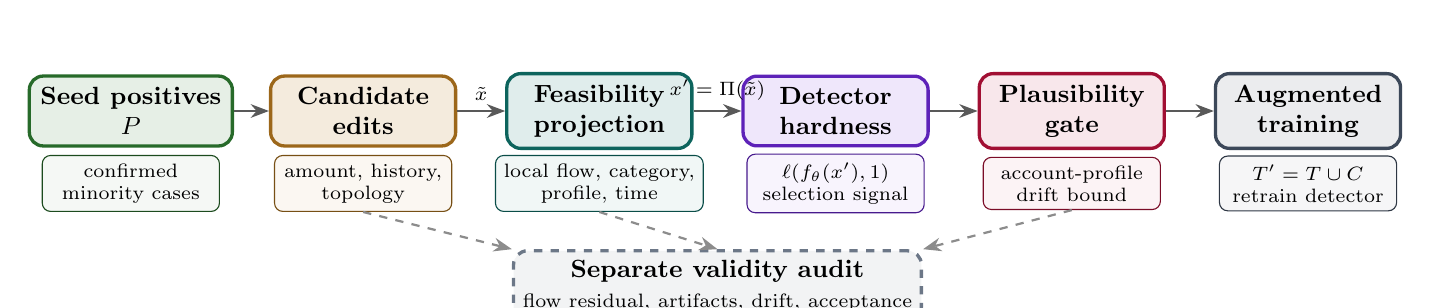
\begin{tikzpicture}[
  stage/.style={rectangle, rounded corners=5pt, very thick, align=center,
                font=\small\bfseries, minimum width=2.35cm, minimum height=0.82cm,
                inner sep=4pt},
  detail/.style={rectangle, rounded corners=3pt, align=center,
                 font=\scriptsize, minimum width=2.25cm, minimum height=0.58cm,
                 inner sep=3pt},
  auditbox/.style={rectangle, rounded corners=5pt, dashed, very thick,
                   draw=FlowSlate!80, fill=FlowSlate!7, align=center,
                   font=\small\bfseries, minimum width=4.9cm, minimum height=0.85cm},
  arr/.style={-Stealth, thick, draw=black!65},
  darr/.style={-Stealth, thick, dashed, draw=black!45}
]
  \node[stage, draw=FlowGreen!85!black, fill=FlowGreen!12] (seed) at (0,0)
        {Seed positives\\$P$};
  \node[detail, draw=FlowGreen!60!black, fill=FlowGreen!5] at (0,-0.92)
        {confirmed\\minority cases};

  \node[stage, draw=FlowAmber!85!black, fill=FlowAmber!15] (edit) at (2.95,0)
        {Candidate\\edits};
  \node[detail, draw=FlowAmber!65!black, fill=FlowAmber!6] (editd) at (2.95,-0.92)
        {amount, history,\\topology};

  \node[stage, draw=FlowTeal!85!black, fill=FlowTeal!13] (proj) at (5.95,0)
        {Feasibility\\projection};
  \node[detail, draw=FlowTeal!65!black, fill=FlowTeal!6] (projd) at (5.95,-0.92)
        {local flow, category,\\profile, time};

  \node[stage, draw=FlowPurple!85!black, fill=FlowPurple!11] (score) at (8.95,0)
        {Detector\\hardness};
  \node[detail, draw=FlowPurple!65!black, fill=FlowPurple!5] at (8.95,-0.92)
        {$\ell(f_\theta(x'),1)$\\selection signal};

  \node[stage, draw=FlowRose!85!black, fill=FlowRose!10] (gate) at (11.95,0)
        {Plausibility\\gate};
  \node[detail, draw=FlowRose!65!black, fill=FlowRose!5] (gated) at (11.95,-0.92)
        {account-profile\\drift bound};

  \node[stage, draw=FlowSlate!85!black, fill=FlowSlate!11] (train) at (14.95,0)
        {Augmented\\training};
  \node[detail, draw=FlowSlate!65!black, fill=FlowSlate!5] at (14.95,-0.92)
        {$T'=T\cup C$\\retrain detector};

  \node[auditbox] (audit) at (7.45,-2.22)
        {Separate validity audit\\\normalfont\scriptsize flow residual, artifacts, drift, acceptance};

  \draw[arr] (seed) -- (edit);
  \draw[arr] (edit) -- node[above, font=\scriptsize] {$\tilde{x}$} (proj);
  \draw[arr] (proj) -- node[above, font=\scriptsize] {$x'=\Pi(\tilde{x})$} (score);
  \draw[arr] (score) -- (gate);
  \draw[arr] (gate) -- (train);
  \draw[darr] (editd.south) -- (audit.north west);
  \draw[darr] (projd.south) -- (audit.north);
  \draw[darr] (gated.south) -- (audit.north east);
\end{tikzpicture}
\caption{Two-column schematic of \fcca. Candidate edits are intentionally local
and detector-driven, but only become training examples after feasibility
projection and profile plausibility gating. The audit below the pipeline is not
a training loss; it is a separate measurement of whether generated examples
remain usable as financial transaction records.}
\Description{Pipeline diagram showing seed positives flowing through candidate
edits, feasibility projection, hardness scoring, plausibility gating, and
training selection, with a separate validity audit attached to generation
stages.}
\label{fig:pipeline}
\end{figure*}

Figure~\ref{fig:pipeline} shows the \fcca pipeline. The design separates three
roles that are usually conflated in augmentation papers. \emph{Candidate
generation} makes examples hard for the current detector; \emph{feasibility
projection} repairs them into auditable transaction records; and a
\emph{separate validity audit} reports artifact rates and profile drift
without folding them into the training signal. This decoupling is what makes
it possible to identify methods that improve scores by exploiting invalid
artifacts (such as unprojected adversarial perturbations) and distinguish
them from methods that improve scores through valid hard support. The core
algorithmic components are the closed-form projection operator
(Algorithm~\ref{alg:project}) and the generation procedure
(Algorithm~\ref{alg:generate}).

\subsection{Perturbation}

Starting from a seed positive transaction $x \in P$, a candidate $\tilde{x}$
is generated by perturbing three complementary feature groups:

\begin{enumerate}
\item \textit{Amount perturbation:} $\tilde{a} = a \cdot (1 + \epsilon_a)$
      where $\epsilon_a \sim \mathcal{U}(-\sigma_{\text{amt}}, \sigma_{\text{amt}})$
      scaled to the empirical amount spread of positive examples.
\item \textit{History perturbation:} Aggregated features (\eg rolling
      transaction count, inflow sum, neighbour degree) are perturbed within
      a configurable profile-width multiplier.
\item \textit{Boundary-mode perturbation:} For hard and typology-aware
      variants, feature-direction gradients from the trained detector
      $f_\theta$ are used to move the candidate towards the positive-class
      region, maximising detector loss.
\end{enumerate}

For the typology-projected variant, perturbation magnitudes are weighted
by feature importance under that typology: layering examples emphasise
multi-hop-flow features and chain-length statistics; structuring emphasises
repeated-small-amount patterns.
These weights are fixed from analyst-specified feature groups and training-time
metadata, not estimated from held-out target positives. This makes the
typology-projected row an analyst-prior setting rather than a zero-knowledge
emerging-typology setting. We therefore also report hard and curriculum
projected variants that do not rely on target-typology weights.

\subsection{Feasibility Projection}

The feasibility projection maps an arbitrary perturbed candidate
$\tilde{x} \in \mathbb{R}^d$ to the nearest point in the validity space,
solving four sub-problems in sequence.

\textbf{Local flow-balance projection.}
Let $\tilde{a}_e$ be the perturbed amount for transaction $e$ originating from
account $v$. Define the row-sum normalisation:
\begin{equation}
  a'_e = \tilde{a}_e \cdot \frac{\sum_{e' \in \text{in}(v)} a_{e'}}
                                  {\sum_{e' \in \text{out}(v)} \tilde{a}_{e'}},
  \label{eq:flowbalance}
\end{equation}
which ensures $\sum_{\text{out}(v)} a'_e = \sum_{\text{in}(v)} a_{e'}$
within the edited local account context. This removes the audited amount
residual for the generated transaction, but it is not a global conservation
operator over all graph edges.

\textbf{Categorical repair.}
Each categorical one-hot block is repaired by setting the maximum-valued
dimension to one and all others to zero:
\begin{equation}
  c'_k = \mathbf{1}[k = \arg\max_j \tilde{c}_j], \quad k = 1, \ldots, K.
  \label{eq:cat}
\end{equation}

\textbf{Profile constraint projection.}
Each account-history dimension $j$ is clipped:
\begin{equation}
  h'_j = \mathrm{clip}\!\left(\tilde{h}_j;\,
    \mu_{v,j} - k\sigma_{v,j},\; \mu_{v,j} + k\sigma_{v,j}\right).
  \label{eq:profile}
\end{equation}
Negative-valued features (\eg transaction counts) are additionally floored
at zero.

\textbf{Temporal feasibility.}
The perturbed timestamp is clamped to the valid window:
\begin{equation}
  t' = \mathrm{clip}(\tilde{t};\, t_{\min}^{(v)},\, t_{\max}^{(v)}).
  \label{eq:temporal}
\end{equation}

The composed projection is $\text{Proj}(\tilde{x}) = (a', c', h', t')$.
By construction, $\text{Proj}(\tilde{x})$ satisfies all four audited local
validity constraints simultaneously.

\begin{algorithm}[t]
\caption{FeasibilityProject}
\label{alg:project}
\begin{algorithmic}[1]
\Require Perturbed candidate $\tilde{x}$; account stats $\{\mu_v, \sigma_v\}$;
         profile width $k$
\Ensure  Validity-compliant projected example $x'$
\State $a' \leftarrow$ LocalFlowBalance$(\tilde{a})$ \Comment{Eq.~\ref{eq:flowbalance}}
\State $c' \leftarrow$ ArgmaxOneHot$(\tilde{c})$ \Comment{Eq.~\ref{eq:cat}}
\State $h' \leftarrow \mathrm{clip}(\tilde{h};\, \mu_v - k\sigma_v,\, \mu_v + k\sigma_v)$ \Comment{Eq.~\ref{eq:profile}}
\State $h' \leftarrow \max(h', \mathbf{0})$ \Comment{Non-negativity}
\State $t' \leftarrow \mathrm{clip}(\tilde{t};\, t_{\min}^{(v)},\, t_{\max}^{(v)})$ \Comment{Eq.~\ref{eq:temporal}}
\State \Return $x' \leftarrow (a', c', h', t')$
\end{algorithmic}
\end{algorithm}

\subsection{Plausibility Gating}
\label{subsec:plausibility}

The plausibility score of a projected example $x'$ is defined as:
\begin{equation}
  S_p(x') = \exp\!\left(-\lambda \cdot \text{drift}(x', \mu_v)\right),
  \label{eq:plausibility}
\end{equation}
where $\text{drift}(x', \mu_v) = \|x'_h - \mu_v\|_2 / \|\sigma_v\|_2$
is the normalised profile deviation, and $\lambda > 0$ is a decay
parameter. A candidate is accepted if $S_p(x') > \tau$, \ie if its
normalised profile deviation is below $-\log(\tau)/\lambda$.
Plausibility gating reduces behavioural implausibility. The validity audit in
Table~\ref{tab:validity_compact} shows the intended tradeoff: projected
variants remain hard for the detector, while plausibility-aware selection
lowers account-profile drift.

\subsection{Typology-Aware Generation and Curriculum}
\label{subsec:typology}

\textbf{Typology-projected variant.}
The typology-projected variant adapts feature-perturbation weights
$w^{(\text{typ})} \in \mathbb{R}^d$ according to the target typology.
For layering, weights are elevated for multi-hop flow features and
chain-length statistics that characterise funds passing through
multiple intermediary accounts. Generation proceeds using the
weighted perturbation, then applies the full feasibility projection.

\textbf{Curriculum projected variant.}
Rather than selecting only maximally hard examples, the curriculum variant
schedules hardness monotonically across epochs: early rounds favour
moderate-hardness examples (hardness score below the 50th percentile of
the current candidate pool); later rounds shift towards the top-hardness
region. This reduces catastrophic boundary distortion in early training,
particularly for typologies (\eg structuring) where the positive-class
boundary is subtle and high-hardness examples from the full positive set
are unrepresentative.

\begin{algorithm}[t]
\caption{\fcca CounterfactualGenerate}
\label{alg:generate}
\begin{algorithmic}[1]
\Require Positive seed set $P$; detector $f_\theta$; augmentation ratio
         $\rho$; candidate-pool multiplier $M$; typology $\tau$;
         plausibility threshold $\tau_p$; account statistics
         $\{\mu_v,\sigma_v\}$
\Ensure  Augmentation set $C$ with $|C|\!\leq\!\lfloor \rho |P|\rfloor$
\State $\mathcal{Q}\leftarrow\emptyset$; \;
       $n_{\text{aug}}\leftarrow\lfloor \rho |P|\rfloor$
\For{each $x \in P$, repeated $M$ times}
    \State $\tilde{x}\leftarrow \mathrm{Perturb}(x, w^{(\tau)})$
           \Comment{typology-weighted edit}
    \State $x'\leftarrow \mathrm{FeasibilityProject}(\tilde{x})$
           \Comment{Algorithm~\ref{alg:project}}
    \State $h\leftarrow \ell(f_\theta(x'), 1)$
           \Comment{detector-loss hardness}
    \State $S_p(x')\leftarrow \exp(-\lambda\,\mathrm{drift}(x',\mu_v))$
           \Comment{plausibility, Eq.~\ref{eq:plausibility}}
    \If{$S_p(x') > \tau_p$ and $x'$ passes validity audit}
        \State $\mathcal{Q}\leftarrow \mathcal{Q}\cup\{(x', h)\}$
    \EndIf
\EndFor
\State Sort $\mathcal{Q}$ by $h$ in descending order (or by curriculum schedule)
\State $C \leftarrow$ top-$n_{\text{aug}}$ items of $\mathcal{Q}$
\State \Return $C$
\end{algorithmic}
\end{algorithm}

%% ============================================================
\section{Experimental Setup}
\label{sec:setup}
%% ============================================================

The experimental design follows four questions: (i) do common augmentations
produce transaction records that pass a financial-validity audit; (ii) does
post-hoc repair of the failing artifacts match validity-aware counterfactual
generation; (iii) does valid hard support actually improve ranking and
alert-budget metrics under a strict emerging-typology protocol; and (iv) where
does the method fail, and what do those failures say about the geometry of the
target typology?

\textbf{Datasets.}
We use three transaction-graph benchmarks (Table~\ref{tab:datasets}). AMLNet
is the primary benchmark because it contains typology labels for layering,
structuring, and integration, which make held-out typology transfer possible.
TransXion is larger and exposes richer account-profile features; we use it as a
full-data robustness check rather than for typology transfer because it has no
public typology labels. Elliptic++ serves as an external predictive sanity
check; we do not run the full validity audit on it because its public feature
schema does not expose the local-flow and profile fields the audit requires.

\begin{table}[t]
\centering
\caption{Transaction-graph benchmarks. The validity audit is only fully
applicable on datasets that expose local-flow and account-profile fields.}
\label{tab:datasets}
\setlength{\tabcolsep}{4pt}
\renewcommand{\arraystretch}{1.08}
\small
\begin{tabular}{@{}lrrcc@{}}
\toprule
\textbf{Dataset} & \textbf{\#Tx} & \textbf{\#Pos} & \textbf{Typology labels} & \textbf{Full audit} \\
\midrule
AMLNet      & 1.09M & 1{,}728 & yes & yes \\
TransXion   & 3.01M & 4{,}631 & no  & yes \\
Elliptic++  & 0.20M & 4{,}545 & no  & no  \\
\bottomrule
\end{tabular}
\end{table}

\textbf{Typology-transfer protocol.}
For held-out typology transfer, all positives of the target typology are
removed from the chronological training split. The detector is trained on the
remaining stream; counterfactuals are generated only from positives available
in that training split; and evaluation is restricted to future positives of
the held-out typology. Layering is the primary positive setting because it has
enough support for ten-seed bootstrap evaluation and the local-flow
counterfactual family matches its dominant signal. Structuring and integration
follow the same protocol as boundary-condition tests.

\textbf{Detectors and baselines.}
The headline detectors are LightGBM~\cite{ke2017lightgbm} and
XGBoost~\cite{chen2016xgboost}, which are strong, stable, and widely deployed
on tabular transaction features. We also include PyG
GraphSAGE~\cite{hamilton2017inductive} and GAT~\cite{velickovic2018graph} as
graph-model checks, reported as limitations rather than secondary wins.
Baselines are grouped by purpose: \emph{no augmentation} measures the detector
alone; \emph{feature noise}, \emph{SMOTE}~\cite{chawla2002smote}, and
\emph{mixup}~\cite{zhang2018mixup} stand in for standard feature-space
augmentation; their \emph{repaired} variants remove audited surface artifacts
post-hoc; \emph{random feasible} augmentation isolates validity without
hardness; and \emph{unprojected adversarial} augmentation is a validity stress
test rather than a competitive baseline. Our pipeline yields three variants:
\emph{hard projected}, \emph{curriculum projected}, and \emph{typology
projected}, each with an optional \emph{plausible} sub-variant that adds
profile-drift gating.

\textbf{Training protocol.}
Each seed runs the same loop: train the base detector on the typology-held-out
split; generate candidates from the available positives; repair or project them
according to the method; select candidates by detector hardness when
applicable; and retrain on the augmented set. Final transfer runs use
augmentation ratio $\rho{=}0.75$, a candidate pool $8{\times}$ larger than the
selected set, log-normal amount perturbation capped at the 99.5th seed-amount
percentile, and method-specific log-normal scales tuned once on a
validity-audit grid and frozen for all reported runs. Candidate selection
requires normalized flow residual $\leq 0.03$. Plausible variants additionally
keep candidates below the 60th profile-drift percentile and the 80th
edit-distance percentile of the candidate pool; the curriculum variant uses a
90th-percentile profile gate and schedules hardness from moderate to high-loss
candidates across epochs.

\textbf{Metrics and reporting.}
The primary predictive metric is AUPRC~\cite{davis2006relationship}, which is
appropriate for severely imbalanced detection. Because AML systems operate
under analyst capacity, we additionally report low-FPR recall and top-alert
precision. \emph{Validity} is evaluated on a separate axis through artifact
rates, audited flow residual, profile drift, candidate acceptance, and
detector hardness. The main held-out layering experiment uses ten random
seeds and a prediction-level paired bootstrap with 200 resamples per seed;
these seeds capture detector and augmentation stochasticity on a fixed
chronological split. All comparisons are paired: for a fixed detector and seed,
the same chronological split, negative population, and evaluation positives are
reused across methods, so the relevant quantity is the change induced by
augmentation rather than absolute AUPRC. We treat invalid-but-predictive,
valid-but-uninformative, and valid-and-hard augmentations as three distinct
outcomes, and require the proposed methods to improve against both
random-feasible and repaired feature-space controls before reporting a
positive result.

\textbf{Implementation and reproducibility.}
Boosted-tree detectors are trained with $1{,}000$ rounds, learning rate
$0.05$, max depth $8$, and class-weighted loss (positive weight set to the
inverse positive rate of the training split). For PyG GraphSAGE and GAT we
use two layers, 64 hidden units, dropout 0.3, Adam at lr $10^{-3}$, and
neighbor sampling with fan-out $(20,10)$; training is run for $100$ epochs
with early stopping on a held-in validation slice. Counterfactual generation
samples $M{=}8$ candidates per positive, applies the projection in
Algorithm~\ref{alg:project}, and computes the hardness score with a single
forward pass through the trained base detector. The profile drift used in
plausibility gating is $\|x'_h-\mu_v\|_2/\|\sigma_v\|_2$ averaged across
account-history dimensions, with $\lambda$ in Eq.~\ref{eq:plausibility} fixed
to $1.0$. Audited flow residual is $|\Delta_{\text{out}}(u)-\Delta_{\text{in}}(v)|$
on the edited transaction. All experiments run on a single CPU node with
$96$ GB RAM; the entire ten-seed held-out layering grid (no-augmentation plus
all augmentation variants, both detectors, all stress slices) completes in
under $9$ wall-clock hours.

%% ============================================================
\section{Results}
\label{sec:results}
%% ============================================================

Section~\ref{subsec:validity} reports the validity audit and shows that
predictive hardness and financial validity are nearly decorrelated across
augmentation families. The held-out layering result is reported as a paired
comparison (\S\ref{subsec:layering}), evaluated at operational alert budgets
(\S\ref{subsec:alert_budget}), and stress-tested under few-shot, temporal,
and new-counterparty slices (\S\ref{subsec:robustness_slices}). Boundary
conditions on non-layering typologies and graph neural detectors are
reported in \S\ref{subsec:boundary_conditions}.

\subsection{Validity Is A Separate Evaluation Axis}
\label{subsec:validity}

Table~\ref{tab:validity_compact} reports predictive hardness and financial
validity as separate measurements. The two axes are nearly decorrelated
across augmentation families. Feature noise violates multiple constraints
simultaneously (58.2\% local-flow violations, 49.9\% categorical artifacts,
35.2\% impossible negative values); unprojected adversarial perturbations are
nominally hard but achieve their hardness by leaving the feasible transaction
space (96.9\% local-flow violation rate). Post-hoc repair removes audited
surface artifacts but collapses detector hardness: repaired SMOTE drops to a
hardness of $0.27$, indistinguishable from no augmentation. Random feasible
augmentation passes the audit but is almost trivial for the detector
($0.03$ hardness). Only the projected variants occupy the region the pipeline
targets: audited validity at hardness $6$--$7$, with substantially lower
profile drift once plausibility gating is added.

\begin{table}[t]
\centering
\caption{Validity audit on generated examples. Invalidity reports nonzero
audited failure signals; ``valid'' means no audited surface artifact. Feature
noise and unprojected adversarial augmentation are stress tests, while repaired
and random-feasible rows are the meaningful controls.}
\label{tab:validity_compact}
\setlength{\tabcolsep}{3pt}
\renewcommand{\arraystretch}{1.08}
\resizebox{\columnwidth}{!}{%
\begin{tabular}{@{}lccc@{}}
\toprule
\textbf{Method family} & \textbf{Invalidity signal} &
\textbf{Hard.} & \textbf{Drift} \\
\midrule
Feature noise & 58.2 L / 49.9 C / 35.2 N & 2.43 & 2.08 \\
Unprojected adversarial & 96.9 L / 0.461 residual & 2.60 & 0.68 \\
SMOTE + repair & valid & 0.27 & 1.46 \\
Mixup + repair & valid & 1.48 & 1.08 \\
Random feasible & valid & 0.03 & 1.30 \\
\midrule
Hard projected & valid & 6.21 & 0.53 \\
Typology projected & valid & 7.05 & 0.52 \\
Plausible typology & valid & 5.71 & 0.29 \\
\bottomrule
\end{tabular}}
\vspace{2pt}
\footnotesize L: local-flow violation; C: categorical artifact; N: negative feature.
\end{table}

An augmentation method that improves AUPRC while failing the audit is
detecting its own artifacts rather than future positives, and a method that
passes the audit while producing uninformative examples cannot be expected to
improve detection under emerging-typology shift. The projected family is the
only one that satisfies both conditions, and the predictive comparisons that
follow are evaluated against repaired and random-feasible controls.

A separate observation worth noting is that plausibility gating reduces
profile drift from $0.53$ (hard projected) to $0.29$ (plausible typology)
without proportionally sacrificing hardness ($6.21\!\to\!5.71$). This is the
design target of \S\ref{subsec:plausibility}: gating trades a small amount of
hardness for a substantial reduction in account-profile deviation. In
deployment terms, a generated transaction whose profile statistics deviate
strongly from the source account is exactly the kind of artifact a
human reviewer would flag as implausible even before the detector scored it,
so reducing drift while retaining hardness is desirable on both predictive
and operational grounds.

\subsection{Held-Out Layering Transfer}
\label{subsec:layering}

Table~\ref{tab:main_layering} reports the held-out layering result for four
comparisons: no augmentation, the best repaired feature-space baseline, random
feasible augmentation, and the best projected variant. For LightGBM, the best
projected variant lifts AUPRC from $0.932$ to $0.947$ (paired bootstrap
$[+0.007,+0.025]$, 10/10 seed wins). For XGBoost, the lift is from $0.927$ to
$0.946$ (paired bootstrap $[+0.010,+0.028]$, 10/10 seed wins). Repaired SMOTE
and random feasible augmentation move the mean by at most $+0.005$, with
bootstrap intervals that include zero. The gain is not isolated to AUPRC; it
transfers to operational metrics, with $R$@0.1\%\,FPR rising by
$0.017$--$0.020$ and Precision@500 by $0.013$--$0.015$.

\begin{table}[t]
\centering
\caption{Main held-out layering result. Values are mean$\pm$std over ten seeds.
The control cell reports the best repaired standard augmentation and random
feasible augmentation; the evidence cell reports the paired interval, seed
wins, and alert-budget gains of the best projected method over no augmentation.}
\label{tab:main_layering}
\setlength{\tabcolsep}{3pt}
\renewcommand{\arraystretch}{1.12}
\resizebox{\columnwidth}{!}{%
\begin{tabular}{@{}lcccc@{}}
\toprule
\textbf{Det.} & \textbf{No aug.} & \textbf{Controls} &
\textbf{Best projected} & \textbf{Paired evidence} \\
\midrule
LGB &
$0.932{\pm}0.001$ &
\makecell{repair $0.934{\pm}0.005$\\feasible $0.934{\pm}0.002$} &
\makecell{\textbf{$0.947{\pm}0.002$}\\Typology proj.\\$\Delta=+0.016$} &
\makecell{$[+0.007,+0.025]$\\10--0 wins\\R@0.1 $+0.017$, P@500 $+0.013$} \\
XGBoost &
$0.927{\pm}0.001$ &
\makecell{repair $0.933{\pm}0.005$\\feasible $0.932{\pm}0.002$} &
\makecell{\textbf{$0.946{\pm}0.003$}\\Curriculum proj.\\$\Delta=+0.018$} &
\makecell{$[+0.010,+0.028]$\\10--0 wins\\R@0.1 $+0.020$, P@500 $+0.015$} \\
\bottomrule
\end{tabular}}
\end{table}

Figure~\ref{fig:paired_deltas} plots the per-seed AUPRC gain over no
augmentation. Random feasible augmentation gives the smallest deltas;
repaired feature-space augmentation barely separates from the baseline; the
largest and most stable deltas come from projected hard, curriculum, and
typology variants. Feasibility alone is therefore not predictive of utility:
the useful signal comes from counterfactuals that are simultaneously
\emph{feasible} and close enough to the held-out layering boundary to apply
real pressure on the detector.

\begin{figure*}[t]
\centering
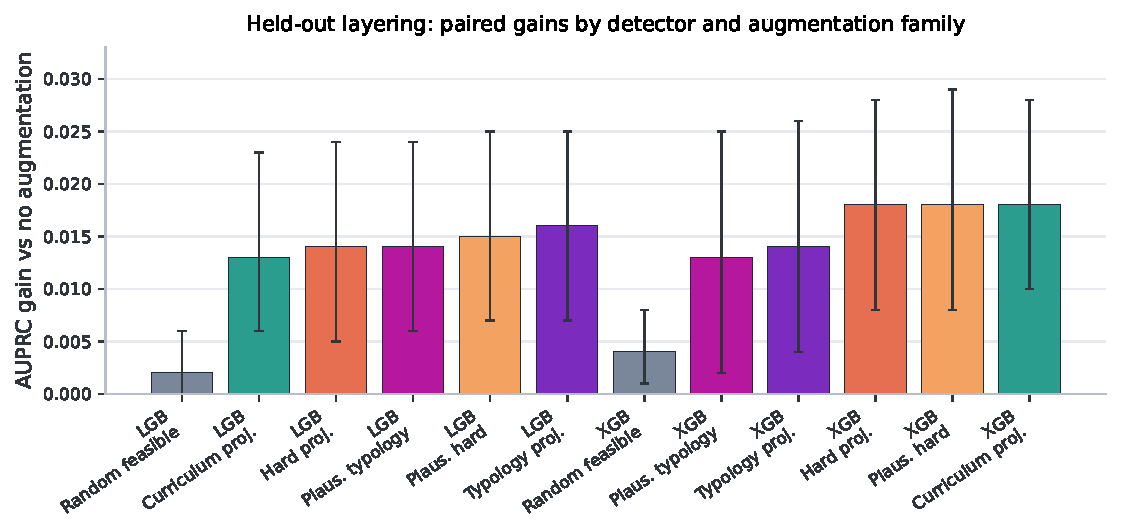
\includegraphics[width=\textwidth]{fig_07_layering_10seed_delta_ci}
\caption{Paired held-out layering AUPRC deltas against no augmentation over ten
seeds. Positive values indicate improvement over the corresponding no-
augmentation detector; error bars show the prediction-level bootstrap interval
summarized across seeds.}
\Description{Bar chart of paired AUPRC deltas for LightGBM and XGBoost
augmentation variants. Projected variants have consistently larger positive
deltas than random feasible augmentation.}
\label{fig:paired_deltas}
\end{figure*}

All comparisons are paired against the same no-augmentation detector and the
same evaluation positives, so the relevant quantity is the change induced by
augmentation rather than absolute AUPRC. Across detectors, the same effect
holds: feasibility produces usable records, while hardness selection is what
moves the future-positive ranking.

\subsection{Paired Bootstrap Significance}
\label{subsec:bootstrap}

Because the absolute AUPRC values on held-out layering are numerically close,
we assess statistical significance with a prediction-level paired bootstrap.
For each detector, seed, and method pair, we resample the test predictions
(positives and negatives) with replacement 200 times and compute the
$\Delta$AUPRC distribution. The 95\% intervals are then summarized across
the ten seeds. Table~\ref{tab:bootstrap} reports the means.

\begin{table}[t]
\centering
\caption{Paired bootstrap intervals on held-out layering ($\Delta$AUPRC),
200 resamples per seed, mean across ten seeds. ``Wins'' is the fraction of
seeds where the lower bound exceeds zero.}
\label{tab:bootstrap}
\setlength{\tabcolsep}{4pt}
\renewcommand{\arraystretch}{1.06}
\small
\begin{tabular}{@{}llccc@{}}
\toprule
\textbf{Det.} & \textbf{Method vs.\ no aug.} &
\textbf{Mean $\Delta$} & \textbf{Bootstrap CI} & \textbf{Wins} \\
\midrule
LGB & SMOTE + repair       & $+0.000$ & $[-0.003,+0.003]$ & 0.6 \\
LGB & Random feasible      & $+0.002$ & $[-0.001,+0.006]$ & 1.0 \\
LGB & Hard projected       & $+0.014$ & $[+0.005,+0.024]$ & 1.0 \\
LGB & Curriculum projected & $+0.013$ & $[+0.006,+0.023]$ & 1.0 \\
LGB & Typology projected   & $\mathbf{+0.016}$ & $[+0.007,+0.025]$ & 1.0 \\
LGB & Plausible typology   & $+0.014$ & $[+0.006,+0.024]$ & 1.0 \\
\midrule
XGB & SMOTE + repair       & $+0.002$ & $[-0.000,+0.005]$ & 1.0 \\
XGB & Random feasible      & $+0.004$ & $[+0.001,+0.008]$ & 1.0 \\
XGB & Hard projected       & $+0.018$ & $[+0.008,+0.028]$ & 1.0 \\
XGB & Curriculum projected & $\mathbf{+0.018}$ & $[+0.010,+0.028]$ & 1.0 \\
XGB & Typology projected   & $+0.014$ & $[+0.004,+0.026]$ & 1.0 \\
XGB & Plausible typology   & $+0.013$ & $[+0.002,+0.025]$ & 1.0 \\
\bottomrule
\end{tabular}
\end{table}

Three observations follow. First, every projected variant has a strictly
positive bootstrap lower bound on both detectors. Second, SMOTE+repair has a
bootstrap interval that includes zero for LightGBM, confirming that the
visible mean gain is not statistically distinguishable from no augmentation.
Third, the projected family separates from random feasible augmentation
(roughly $0.012$--$0.014$ larger $\Delta$, with non-overlapping intervals on
LightGBM), so the improvement cannot be attributed to feasibility alone.

\subsection{Operational Alert Budgets}
\label{subsec:alert_budget}

AML systems are not deployed by sorting an entire benchmark; analysts work
through a capped queue of alerts per period. The paired evidence in
Table~\ref{tab:main_layering} therefore reports changes at low false-positive
and top-alert operating points rather than introducing another full metric
table. The best projected variant raises $R$@0.1\%\,FPR by
$+0.017$ (LightGBM) and $+0.020$ (XGBoost), and Precision@500 by
$+0.013$ and $+0.015$ respectively. Precision@100 is omitted because it
saturates near $1.0$ across nearly all methods and does not discriminate.
Translated to capacity: at a fixed 0.1\%\,FPR alert budget, the projected
variant brings into the alert window roughly two additional held-out layering
positives per hundred actually present compared to the no-augmentation
baseline---a sizeable shift at the scale typical of bank-side AML triage.

\subsection{Stress Tests: Few-Shot, Time, and New Counterparties}
\label{subsec:robustness_slices}

Table~\ref{tab:stress_slices} reports three deployment-relevant slices.
\emph{(i) Few-shot adaptation.} Adding ten confirmed target-typology positives
to the training set narrows the gap but does not eliminate it
($\Delta{=}{+}0.013$/${+}0.012$ for LightGBM/XGBoost): projected augmentation
remains useful after a small number of real positives arrive.
\emph{(ii) Temporal drift.} Bucketing the test stream into time quartiles
shows the largest gain in the earliest future bucket
($\Delta{=}{+}0.083$/${+}0.080$), where the no-augmentation baseline is
weakest. This bucket is the closest analogue to a fresh-deployment regime, in
which an emerging typology has begun appearing but training data has not yet
been refreshed.
\emph{(iii) New counterparties.} Restricting evaluation to future
sender-receiver pairs unseen during training isolates the cold-start regime;
profile-aware projected variants yield the largest improvements
($\Delta{=}{+}0.023$/${+}0.020$). The sparse low-history entity subset
contains only $11$ positives and is omitted from the main table.

\begin{table}[t]
\centering
\caption{Stress tests for held-out layering. Values are AUPRC mean$\pm$std.}
\label{tab:stress_slices}
\setlength{\tabcolsep}{3pt}
\renewcommand{\arraystretch}{1.12}
\resizebox{\columnwidth}{!}{%
\begin{tabular}{@{}llccc@{}}
\toprule
\textbf{Slice} & \textbf{Detector} & \textbf{No aug.} &
\textbf{Best projected} & \textbf{$\Delta$} \\
\midrule
Few-shot & LGB & $0.938{\pm}0.003$ &
$0.951{\pm}0.005$ & $+0.013$ \\
Few-shot & XGB & $0.936{\pm}0.005$ &
$0.948{\pm}0.002$ & $+0.012$ \\
Temporal Q1 & LGB & $0.655{\pm}0.006$ &
$0.738{\pm}0.014$ & $+0.083$ \\
Temporal Q1 & XGB & $0.651{\pm}0.002$ &
$0.731{\pm}0.024$ & $+0.080$ \\
New pair & LGB & $0.928{\pm}0.002$ &
$0.951{\pm}0.005$ & $+0.023$ \\
New pair & XGB & $0.923{\pm}0.001$ &
$0.943{\pm}0.009$ & $+0.020$ \\
\bottomrule
\end{tabular}}
\end{table}

Each slice corresponds to a shift that typically triggers AML model
retraining in practice. The gain is concentrated in the regimes where the
no-augmentation baseline is weakest---earliest future bucket and unseen
counterparties---consistent with the role of projected augmentation as a
label-scarcity mechanism rather than an in-distribution oversampler.
Figure~\ref{fig:scope_map} places these wins alongside the failures of
\S\ref{subsec:boundary_conditions}.

\begin{figure*}[t]
\centering
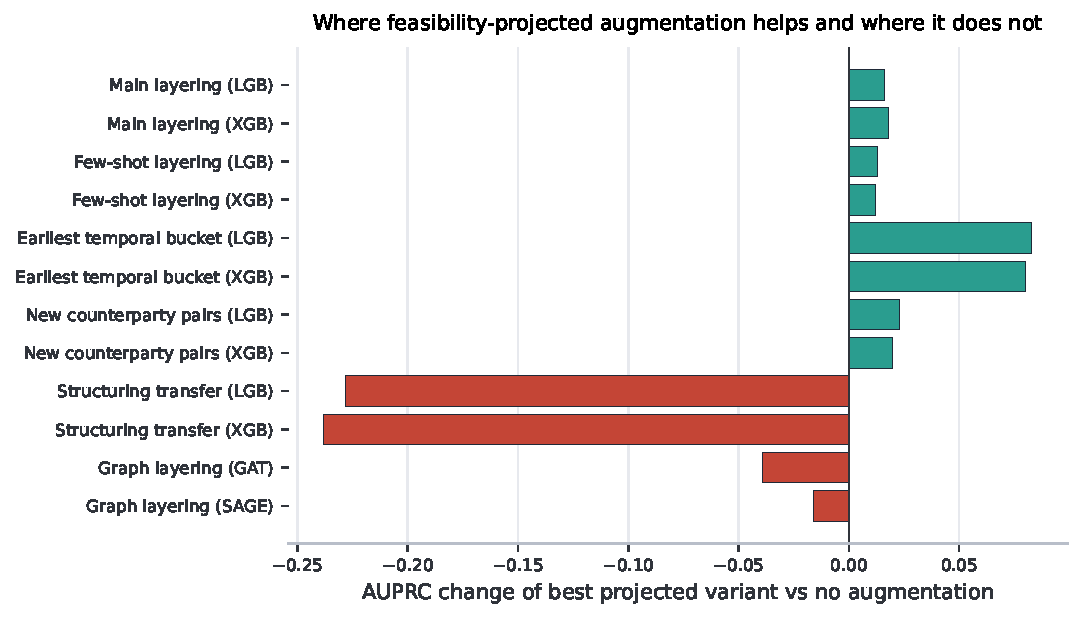
\includegraphics[width=0.92\textwidth]{fig_08_effect_scope_map}
\caption{Scope of the empirical effect. Positive bars are layering settings in
which the best projected variant improves over no augmentation; negative bars
show failure cases where the same family does not transfer.}
\Description{Horizontal diverging bar chart showing positive AUPRC changes for
main layering, few-shot layering, temporal layering, and new-pair layering, and
negative changes for structuring transfer and graph layering checks.}
\label{fig:scope_map}
\end{figure*}

\subsection{Boundary Conditions}
\label{subsec:boundary_conditions}

Figure~\ref{fig:scope_map} reports the negative results. Structuring is the
cleanest case: projected examples remain valid but move the detector toward
the wrong support region, reducing AUPRC from $0.618{\pm}0.041$ to
$0.390{\pm}0.003$ for LightGBM and from $0.625{\pm}0.029$ to
$0.387{\pm}0.006$ for XGBoost. Random feasible augmentation outperforms hard
projection on XGBoost structuring, indicating that the failure is not driven
by invalid examples but by projected support that no longer matches the
held-out structuring region (\S\ref{subsec:mechanism_layering}). Integration
AUPRCs are at the $10^{-4}$ scale across all methods and seeds; we report
only the relative ordering. The PyG GNN check on held-out layering does not
reproduce the boosted-tree improvement: mean AUPRC stays near the baseline
with high seed variance ($0.705{\pm}0.089$ for GAT, $0.355{\pm}0.275$ for
GraphSAGE), suggesting that the local edge edits do not survive neighborhood
aggregation as a clean training signal. \fcca is therefore
typology-sensitive and detector-sensitive, rather than a universal
augmentation recipe.

%% ============================================================
\section{Ablations and Analysis}
\label{sec:mechanism}
%% ============================================================

\subsection{Why Layering Helps But Structuring Fails}
\label{subsec:mechanism_layering}

The most informative diagnostic comes from comparing generated and held-out
examples in feature space. For layering, projection moves generated examples
from a mean nearest-neighbor distance of $1.18$ (random feasible) to $0.73$
(plausible typology) against held-out layering positives, while raising
detector hardness from $0.04$ to $7.95$ (Table~\ref{tab:mechanism}). The
generated log-amounts ($\approx 7.0$) are close to the held-out target
($8.76$). For structuring, NN distance to held-out positives drops similarly
(from $2.34$ to $0.82$) and hardness climbs to $8.19$, but the generated
log-amounts collapse to $5.63$ against a target of $8.58$. Integration is
extreme: generated log-amounts ($\approx 5.9$) sit nearly five orders of
magnitude below the target ($10.90$).

\noindent\emph{Geometric proximity is necessary but not sufficient.} Hard
projected examples are close to held-out positives in standardized feature
space, but ``close'' in standardized coordinates can still mean ``far'' in the
amount regime that defines the typology. For structuring---the canonical
small-amount typology---hard projection drives amounts \emph{downward} below
even the structuring threshold, so the detector is trained on valid hard
examples from the wrong semantic region. This is the cleanest mechanistic
explanation we have for the negative result in
Figure~\ref{fig:scope_map}: feasibility-aware augmentation is a
\emph{support-coverage} method, not a \emph{semantic-typology} method.

\begin{figure}[t]
\centering
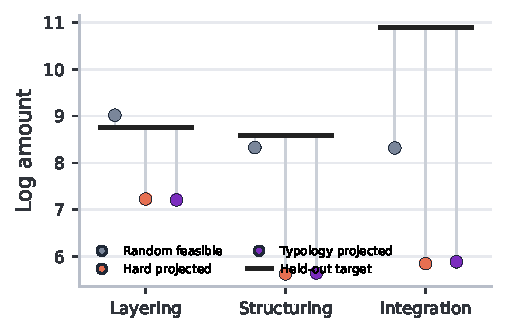
\includegraphics[width=\columnwidth]{fig_09_amount_alignment}
\caption{Amount alignment explains the typology boundary. The black segment
marks the held-out target amount regime; colored points show generated support.
Layering remains close enough to be useful, while projected structuring and
integration examples move into much lower amount regimes.}
\Description{Dot plot comparing generated log amounts with held-out target log
amounts for layering, structuring, and integration.}
\label{fig:amount_alignment}
\end{figure}

\begin{table}[t]
\centering
\caption{Mechanism diagnostics on AMLNet generated examples. NN distance is to
held-out positives in standardized transaction/history feature space.}
\label{tab:mechanism}
\setlength{\tabcolsep}{3pt}
\renewcommand{\arraystretch}{1.08}
\resizebox{\columnwidth}{!}{%
\begin{tabular}{@{}llccccc@{}}
\toprule
\multirow{2}{*}{\textbf{Typology}} & \multirow{2}{*}{\textbf{Method}} &
\multirow{2}{*}{\textbf{NN dist.}} & \multirow{2}{*}{\textbf{Hard.}} &
\multirow{2}{*}{\textbf{Drift}} &
\multicolumn{2}{c}{\textbf{Log amount}} \\
\cmidrule(l){6-7}
& & & & & \textbf{Generated} & \textbf{Target} \\
\midrule
Layering & Random feasible & $1.182{\pm}0.285$ & 0.04 & 2.55 & 9.02 & 8.76 \\
Layering & Hard projected & $0.764{\pm}0.022$ & 9.11 & 1.11 & 7.23 & 8.76 \\
Layering & Plausible typology & $0.726{\pm}0.027$ & 7.95 & 0.85 & 6.97 & 8.76 \\
\midrule
Structuring & Random feasible & $2.341{\pm}0.210$ & 0.03 & 1.77 & 8.33 & 8.58 \\
Structuring & Hard projected & $0.816{\pm}0.020$ & 8.19 & 0.63 & 5.63 & 8.58 \\
Structuring & Typology projected & $0.833{\pm}0.019$ & 8.34 & 0.63 & 5.65 & 8.58 \\
\midrule
Integration & Random feasible & $5.831{\pm}0.080$ & 0.01 & 1.76 & 8.32 & 10.90 \\
Integration & Hard projected & $6.610{\pm}0.023$ & 8.10 & 0.69 & 5.85 & 10.90 \\
Integration & Typology projected & $6.607{\pm}0.020$ & 8.40 & 0.70 & 5.89 & 10.90 \\
\bottomrule
\end{tabular}}
\end{table}

Figure~\ref{fig:amount_alignment} and Table~\ref{tab:mechanism} make this
precise: for structuring and integration, the generated examples are valid
and hard but lie outside the amount regime of the target typology. The
practical implication is that any validity-aware augmentation deployment
should be accompanied by a typology audit comparing the generated and target
amount distributions before committing candidates to training.

\subsection{Constraint Ablations}
\label{subsec:ablations}

Table~\ref{tab:ablations} isolates which constraints and perturbation
families carry the result. Three patterns emerge. First, on AMLNet the
no-flow ablation can raise \emph{raw} AUPRC slightly above the full
projection, but this is not a deployable improvement: the audit shows the
detector is exploiting amount movement that fails the local flow check. This
is precisely the validity gap recovered as an ablation. Second, on TransXion the ordering reverses: profile-removal hurts
sharply (e.g.\ $0.269{\to}0.240$ for LightGBM), and topology-only
perturbation is best. Third, the useful feasible direction is therefore
dataset- and typology-dependent; the validity projection defines the
feasible set, but does not decide which feasible directions are semantically
useful.

\begin{table}[t]
\centering
\caption{Constraint ablation AUPRC (mean $\pm$ std, 3 seeds). Higher raw AUPRC
under no-flow should not be read as a valid improvement; it indicates that
invalid amount movement can be predictive if the model is allowed to exploit
it.}
\label{tab:ablations}
\setlength{\tabcolsep}{3pt}
\renewcommand{\arraystretch}{1.08}
\resizebox{\columnwidth}{!}{%
\begin{tabular}{@{}llccccc@{}}
\toprule
\textbf{Dataset} & \textbf{Det.} & \textbf{Hard proj.} &
\textbf{no-flow} & \textbf{no-profile} &
\textbf{amt.-only} & \textbf{topo.-only} \\
\midrule
AMLNet & LGB &
  $0.977{\pm}0.001$ & $\mathbf{0.980{\pm}0.001}$ &
  $0.978{\pm}0.001$ & $0.974{\pm}0.001$ & $0.971{\pm}0.001$ \\
AMLNet & XGB &
  $0.969{\pm}0.001$ & $0.976{\pm}0.002$ &
  $\mathbf{0.976{\pm}0.002}$ & $0.972{\pm}0.001$ & $0.971{\pm}0.001$ \\
TransXion & LGB &
  $0.269{\pm}0.003$ & $0.262{\pm}0.003$ &
  $0.240{\pm}0.001$ & $0.265{\pm}0.001$ & $\mathbf{0.271{\pm}0.002}$ \\
TransXion & XGB &
  $0.236{\pm}0.004$ & $0.237{\pm}0.006$ &
  $0.230{\pm}0.002$ & $0.242{\pm}0.006$ & $\mathbf{0.248{\pm}0.005}$ \\
\bottomrule
\end{tabular}}
\end{table}

\subsection{Additional Observations}
\label{subsec:additional}

Three further observations are worth noting briefly. \emph{(i) Full-data
AMLNet.} When all typologies are visible during training, projected variants
still narrowly lead on AMLNet ($0.978$ vs.\ $0.971$ no-aug for LightGBM,
Table omitted), but the margin is small enough that the held-out typology
setting remains the more discriminating evaluation.
\emph{(ii) TransXion full-data.} TransXion is closer to a no-shift setting and
favors lightly repaired feature-space augmentation (e.g.\ feature-noise+repair
at $0.280$ for LightGBM, vs.\ $0.272$ no-aug); projected variants do not
improve here, consistent with the support-coverage interpretation---there
is little untouched future-typology region for them to fill.
\emph{(iii) Augmentation ratio.} A sweep over $\rho\in\{0.25,0.5,0.75,1.0\}$
shows the layering result is stable in the $[0.5,1.0]$ band; we fix
$\rho{=}0.75$ for all reported runs. This rules out a narrowly tuned ratio
as the source of the gain.

\FloatBarrier

%% ============================================================
\section{Discussion and Limitations}
\label{sec:discussion}
%% ============================================================

\textbf{Scope of the result.}
Validity-aware counterfactual augmentation improves held-out layering
transfer on the AMLSim-derived benchmark across low-FPR alert budgets,
temporally drifted future data, and previously unseen counterparty pairs,
while repaired feature-space and random-feasible baselines do not. The gain
is consistent across ten seeds, prediction-level paired bootstrap intervals,
two strong boosted-tree detectors, and three deployment-relevant slices. It
does not extend to graph neural detectors or to non-layering AML typologies
under the same per-edge projection family.

\textbf{Asymmetric validity--utility tradeoff.}
Financial validity removes a failure mode of augmentation but does not
guarantee utility. The constraint ablation in
Table~\ref{tab:ablations} shows that dropping the flow constraint sometimes
raises raw AUPRC on the AMLSim-derived dataset because the learner exploits
amount movement that fails the audit. As an in-distribution metric this
appears as a positive ablation; as a deployment metric it is a warning that
augmentation in financial settings should be evaluated on two axes by
default, not one.

\textbf{Why structuring and graph models fail.}
The mechanism analysis identifies two distinct failure modes. For
structuring, the projected support has the right geometric proximity to
held-out positives in standardized feature space, but the amount regime
collapses below the typology's defining threshold; the detector receives hard
examples from the wrong semantic region. For graph neural detectors, the
local edge edits interact with neighborhood aggregation, temporal sampling,
and message propagation in ways the per-edge feasibility projection does not
control. A useful individual transaction record is not necessarily a useful
node or subgraph representation update.

\textbf{Complexity and overhead.}
For a positive seed set of size $|P|$ and pool multiplier $M$, candidate
generation requires $O(M|P|)$ forward passes through the detector for the
hardness score, plus $O(M|P|d)$ time for projection, where $d$ is the feature
dimension. On AMLNet ($|P|\!\approx\!1{,}700$) with $M{=}8$ and $\rho{=}0.75$,
\fcca adds roughly 12--18 seconds of overhead per seed on top of the
LightGBM training time, dominated by detector forward passes. Memory overhead
is negligible because candidates are scored in mini-batches and only the
top-$n_{\mathrm{aug}}$ are retained. The projection itself is closed-form and
introduces no extra trainable parameters.

\textbf{Limitations and future work.}
Three limitations bound the result. \emph{(i)} The AMLSim-derived benchmark
provides the clean typology labels needed for held-out transfer, but it is
synthetic; TransXion is larger and profile-rich but lacks typology
annotations. A natural next step is reproducing the held-out protocol on a
production-derived dataset with confirmed typology labels. \emph{(ii)} The
feasibility projection is closed-form and per-edge; coupling it with a
\emph{typology generator} that reasons over multi-edge episodes, amount
schedules, and temporal spacing should narrow the structuring and
integration gap. \emph{(iii)} Differentiable projection layers and
projection-aware GNN training objectives are an obvious path to making the
same validity mechanism useful for message-passing detectors. Each of these
extensions is consistent with the two-axis evaluation framing introduced
here rather than a departure from it.

%% ============================================================
\section{Conclusion}
\label{sec:conclusion}
%% ============================================================

We argued that augmentation for transaction-graph fraud detection should be
evaluated on \emph{two} axes: predictive utility and financial validity.
\fcca operationalizes this view through a closed-form feasibility projection
that enforces local flow balance, categorical integrity, account-profile
bounds, and temporal feasibility, paired with detector-hardness selection and
profile-drift gating. The evidence is sharpest on held-out layering transfer:
across ten seeds, two boosted-tree detectors, paired bootstrap intervals, and
three deployment-relevant slices, valid projected counterfactuals improve
both AUPRC and operational alert-budget metrics over no augmentation,
repaired SMOTE/mixup, and random-feasible controls. The same family
\emph{does not} improve structuring, integration, or graph neural detectors,
and we explain those failures through a mechanism analysis showing that
geometric proximity in standardized feature space is necessary but not
sufficient---the generated support must also match the semantic geometry of
the target typology. Taken together, the results argue for
typology-sensitive, validity-audited augmentation as a more credible path
for financial fraud detection than unconstrained synthetic generation.

\section*{Reproducibility}
An anonymous reproducibility artifact containing code, configuration files,
processed datasets, processed result tables, plotting scripts, and cached
seed-level outputs is available at
\url{https://github.com/representer-fun/fc-cga-reproducibility}.

\section*{GenAI Usage Disclosure}
The authors used generative AI tools (e.g., ChatGPT) solely for improving the
grammar and clarity of the text. No content, analysis, code, or ideas
generated by AI tools were used in the conception, development, or evaluation
of the research.

\balance

\bibliographystyle{ACM-Reference-Format}
\bibliography{references}

\end{document}
